%%
%% This is file `mcmthesis-demo.tex',
%% generated with the docstrip utility.
%%
%% The original source files were:
%%
%% mcmthesis.dtx  (with options: `demo')
%% 
%% -----------------------------------
%% This is a generated file.
%% 
%% Copyright (C) 2010 -- 2015 by latexstudio
%%       2014 -- 2019 by Liam Huang
%%       2019 -- present by latexstudio.net
%% 
%% This work may be distributed and/or modified under the
%% conditions of the LaTeX Project Public License, either version 1.3
%% of this license or (at your option) any later version.
%% The latest version of this license is in
%%   http://www.latex-project.org/lppl.txt
%% and version 1.3 or later is part of all distributions of LaTeX
%% version 2005/12/01 or later.
%% 
%% The Current Maintainer of this work is latexstudio.net.
%% 
%% !Mode:: "TeX:UTF-8"
\documentclass{mcmthesis}
 %\documentclass[CTeX = true]{mcmthesis}  % 当使用 CTeX 套装时请注释上一行使用该行的设置
\mcmsetup{tstyle = \color{red}\bfseries,  % 修改题号，队号的颜色和加粗显示，黑色可以修改为 black
          tcn = 2625558, problem = B,     % 修改队号，参赛题号
          sheet = true, titleinsheet = true, keywordsinsheet = true,
          titlepage = false, abstract = true}

\usepackage{amsmath}
\usepackage{amssymb}

  %四款字体可以选择
  %\usepackage{times}
  %\usepackage{newtxtext}B
  %\usepackage{palatino}
\usepackage{txfonts}

\usepackage{caption}  
\captionsetup[figure]{font=small}   % 将图标题字号设为small
\captionsetup[table]{font=small}    % 将图标题字号设为small

\usepackage{indentfirst}  % 首行缩进，注释掉，首行就不再缩进
\usepackage{esint}        % 积分号
\usepackage{subcaption}   % 并排图片
\usepackage{floatrow}     % 并排图片
\usepackage{setspace}
\usepackage{float}
\floatstyle{plaintop}
\restylefloat{table}

\usepackage{xcolor}       % 颜色支持
\usepackage{tabularray}   % 增强表格功能

\usepackage[style=numeric,backend=biber]{biblatex}  
\ExecuteBibliographyOptions{sorting=none}           
\addbibresource{references.bib}                     

% 修复fancyhdr警告
\setlength{\headheight}{14pt}
\addtolength{\topmargin}{-1.6pt}  % 可选：保持总版心不变

\setcounter{tocdepth}{2}  % 设置目录到二级标题, 将目录控制在1页
                          % 若可接受目录2页, 注释掉该句, 将到三级标题
                          
\title{The Tether and the Flame: A Multi-Objective Lunar Supply Chain Model}

% \author{\small \href{https://www.latexstudio.net/}
%   {\includegraphics[width=7cm]{mcmthesis-logo}}}

\date{\today}

\begin{document}
\nocite{*} 
\begin{abstract}
\par Neil Armstrong’s "giant leap" opened the door to the cosmos, but establishing a permanent 100,000-person Moon Colony requires us to walk through it with industrial-scale logistics. To manage the colossal transport of 100 million metric tons, we balance the “Tether” of \textbf{space elevators} against the “Flame” of \textbf{rocketry}. This paper constructs a multi-objective framework integrating queueing theory, robust optimization, and environmental assessment to determine the optimal supply chain architecture for lunar civilization.

We evaluate three transportation architectures. For the Space Elevator, we model utilization-dependent congestion costs using \textbf{queueing theory} and account for capacity losses due to tether sway. For Rockets, we derive \textbf{latitude-corrected} payload capacity via \textbf{the Tsiolkovsky equation} and capture cost reduction trends with \textbf{the Wright Learning Curve}. Under the constraint of achieving the minimum completion time, a Hybrid Optimization model yields the optimal allocation fraction $\alpha$, and the minimum cost is achieved at $\alpha = 0.71$.

To account for volatility, we introduce a \textbf{Risk-Adjusted Utility Metric} utilizing Monte Carlo simulations to model failures and groundings. Sensitivity analysis reveals a strategic trade-off: expanding rocket capacity five-fold unlocks a “Fast Track” strategy. This reduces the timeline by ~33\% but doubles the risk-adjusted cost, explicitly quantifying the premium paid for speed over stability.

We design a Dynamic Water Resource Management Scheme using a modified exponential model $r(t)$ for recycling efficiency (50\%--95\%). Coupling this with a convex cost model, our \textbf{Phased Water Management Strategy} reduces total logistics costs by 15\% compared to static demand by delaying high consumption until recycling matures.

Our Environmental Impact Assessment uses Principal Component Analysis (PCA) to aggregate emissions ($CO_2, SO_2, NO_x, BC$) into a composite Environmental Pressure (EP) score. By analyzing the system's sensitivity to a weighting parameter $\omega$, we identify a structural transition to cleaner operations—a "Green Shift"—at the tipping point $\omega_1 \approx 0.08$. However, even under strict constraints, the optimal strategy saturates at a hybrid mix ($\alpha \approx 0.6$) due to elevator throughput bottlenecks.

The strength of this study lies in the \textbf{holistic integration} of non-linear logistics (congestion, learning curves) and stochastic risks, offering higher fidelity than static linear models, despite the unavoidable reliance on projected 2050 parameters. We also acknowledge that aggregating complex ecological impacts into scalar metrics may obscure localized nuances.

Consequently, we recommend prioritizing the Space Elevator as the logistics backbone, reserving rockets for surge capacity. Strategic investments should focus on expanding elevator throughput rather than merely reducing rocket costs to achieve a sustainable "Green Moon" supply chain.

\begin{keywords}
Space Elevator, Wright Learning Curve, Robust Optimization, Monte Carlo Simulation, PCA Environmental Assessment, Dynamic Water Recycling
\end{keywords}

\end{abstract}
\maketitle

%% Generate the Table of Contents, if it's needed.
\begin{spacing}{0.9}
\tableofcontents
\end{spacing}
\newpage

\section{Introduction}
\subsection{Problem Background}

\par Establishing a permanent lunar settlement represents a shift from short-term exploration to large-scale space infrastructure development. This transition demands long-haul, high-volume Earth–Moon transportation systems with high reliability, continuity, and environmental sustainability.
\par Chemical rockets have enabled space access and lunar missions. While mature and flexible, they face inherent limits in cost efficiency, launch frequency, and environmental footprint when scaled for sustained lunar habitation, driving interest in alternative architectures.
\par The proposed Space Elevator System offers a distinct paradigm: continuous, electrically powered transport via ultra-long tethers from Earth’s surface to geosynchronous orbit and beyond. Paired with equatorially distributed Galactic Harbours, it can act as a long-term logistics backbone for large-scale space construction.
\par Rockets and space elevators are complementary strategic options rather than mutually exclusive solutions. Their differences in scalability, operational risk, and environmental impact provide key criteria for planning sustained lunar development.

\subsection{Restatement of the Problem}

The goal of this problem is to develop a quantitative model to support the construction and long-term sustainability of a 100,000-person Moon Colony, requiring the transportation of 100 million metric tons of materials from Earth to the Moon.
Specifically, the following problems are addressed:
 
\begin{itemize}
\item {\bf Problem 1:} Model and compare three material transportation strategies,\\
 (a) exclusive use of the Space Elevator System with three Galactic Harbors,\\
 (b) exclusive use of traditional rocket launches from existing Earth-based facilities,\\
 (c) a hybrid strategy combining both methods.
\item {\bf Problem 2:} Incorporate non-ideal operating conditions, such as system failures and operational disruptions, to assess the robustness and reliability of each transportation strategy.
\item {\bf Problem 3:} Estimate the one-year water demand of a fully operational Moon Colony and analyze the additional cost and time required to deliver this water using the proposed transportation models.
\item {\bf Problem4:} Evaluate the environmental impacts on Earth under each scenario and adjust the model to reduce environmental damage while maintaining feasibility.
\item {\bf Problem5:} Synthesize model results to recommend an optimal course of action to the fictional MCM Agency for building and sustaining the Moon Colony.
\end{itemize}

\subsection{Our work}

\begin{figure}[H]    % H表示强制固定在当前位置
\small
\centering
\includegraphics[width=0.81\textwidth]{fig 1.jpg}
\caption{Our work} \label{fig1}
\end{figure}

\indent First, we develop a unified cost–capacity framework to compare three transportation architectures (space elevator, rockets, and a hybrid system), and solve for the optimal allocation share $\alpha$ via hybrid optimization.

\indent Second, we introduce a Monte Carlo–based risk-adjusted utility metric that explicitly accounts for failures and groundings, and conduct sensitivity analysis to quantify the trade-off between speed and stability.

\indent Third, we design a dynamic water resource management model and propose a phased consumption strategy that leverages improving recycling efficiency to reduce overall logistics cost.

\indent Finally, we evaluate the optimal policy under ecological threshold constraints, explaining why the solution remains hybrid and is ultimately limited by space-elevator throughput bottlenecks.

\section{Assumptions and Justifications}
\begin{itemize}\item {\bf Assumption:} No technological explosion will occur by 2050, and current data can be used to predict relevant indicators for the next 50 years.\item {\bf Justification:} Technological development is a gradual process requiring long-term accumulation and iteration. Predicting future parameters based on existing aerospace data ensures the model’s rationality and feasibility.\item {\bf Assumption:} Pollution from the space elevator is negligible.\item {\bf Justification:} The space elevator produces no atmospheric pollution, and rocket fuel consumption from the apex anchor to the Moon is drastically reduced. Its overall pollution is far lower than that of traditional rockets.\item {\bf Assumption:} Water recycling efficiency will gradually improve over time.\item {\bf Justification:} In the early lunar base operation, water recycling systems are incomplete, and infrastructure construction demands large water volumes. System optimization takes time, so a gradual efficiency increase aligns with real-world operational patterns.\item {\bf Assumption:} The lunar base population remains stable at 100,000.\item {\bf Justification:} In the short term, births and deaths are negligible relative to the total population, simplifying calculations of daily water and material demand.\end{itemize}

\section{Notations}

The key mathematical notations used in this paper are listed in Table \ref{tbl1}. 

%% 三线表
\begin{table}[H]     % H表示强制固定在当前位置
\small
\centering           % 设置居中
\caption{Notations}  % 表标题
\label{tbl1}         % 设置表的引用标签
\begin{tabular}{clc}  % 3列, c表示居中对齐, l和r表示左右对齐
\toprule             % 画顶端横线
{\bf Symbol}    &  {\bf Definition}   & {\bf Unit}\\
\midrule             % 画中间横线
$L_1$          & Payload capacity              & tons/year\\
$L_2$          & Payload capacity              & tons/launch\\
$C_1$          & Space elevator transportation cost  & \$/ton\\
$C_2$          & Rocket launch and delivery cost  & \$/launch\\
$u$            & Allowable utilization rate & - \\
$T$          & Project duration               & years\\
$M$          & Total material transport volume  & tons\\
$F$          & Annual fixed cost    & \$/year\\
$\kappa$          &Transport load factor &\$/tons\\
$N$          & Number of launches per year    & /year\\
$\phi$       & Launch site latitude    & degree$(^{\circ})$\\
$b$          & Wright learning curve exponent    & -\\
$\lambda_{break}$          & Annual frequency of failures   & /year\\
$\eta$       & Operational availability factor    & -\\
$J$          & Risk-adjusted cost metric    & \$\\
$r$          & Water recycling efficiency    & -\\

\bottomrule         % 画底部横线
\end{tabular}
\vspace{2pt} % 稍微调整间距
\begin{flushleft} \small
$^{*}$ There are some variables that are not listed here and will be discussed in detail in each
section.
\end{flushleft}
\end{table}

\section{Data Collection}
\label{sec:data}

All values use \textbf{constant USD (no inflation)}, with 2050 projections incorporating technology maturity (via Wright learning curves) instead of CPI escalation.


\subsection{Economic Parameters}
\begin{itemize}
\item \textbf{Rockets}: 
  Per-launch cost $C_2$: $1.2\times 10^8$ USD/launch (from SpaceX Falcon Heavy public pricing, 2025);
  Annual fixed cost $F_2$: 1.6 B USD/year (from NASA launch site operation budgets, 2020)
\item \textbf{Space Elevator}: 
  Earth$\rightarrow$Apex unit cost $C_{E-A}$: 20 USD/kg (from ISEC space elevator feasibility reports, 2023);
  Apex$\rightarrow$Moon unit cost $C_{A-M}$: 150 USD/kg (from ISEC space elevator feasibility reports, 2023);
  Total unit cost $C_1 = C_{E-A} + C_{A-M}$: $1.0\times 10^5$ USD/ton (estimated);
  Annual maintenance cost $F_1$: 1.0 B USD/year (from large-scale infrastructure maintenance benchmarks, 2024)
\end{itemize}


\subsection{Launch Cadence}
\begin{itemize}
\item 10 launch sites: Empirical launch shares $\omega_i = h_i/\sum h_j$ (from 2025 global orbital launch statistics, total baseline launches $\sum h_j = 234$, $h_i$ = site-level launches);
\item 2050 total maximum launch capacity: $N_{\text{total}}^{\max} = 2000$ launches/year (projected based on 2025--2050 global aerospace infrastructure expansion);
\end{itemize}


\subsection{Reliability/Risk Parameters}
\begin{itemize}
\item \textbf{Space Elevator}: 
  Swaying time fraction $P_{sway}$: 0.10 (from tether dynamics simulations, ISEC 2023);
  Capacity factor during sway $\beta$: 0.8 (from tether dynamics simulations, ISEC 2023);
  Annual breakdown frequency $\lambda_{break}$: 0.05 /year (from large-scale aerospace system failure data, 2022);
  Mean repair time $T_{repair}$: 30 days (from large-scale aerospace system failure data, 2022);
  Cost per repair event $C_{unit}$: 0.2 B USD (from large-scale aerospace system failure data, 2022)
\item \textbf{Rockets}: 
  Launch failure probability $P_{fail}$: 0.01/0.03 (from ESA/NASA launch reliability reports, 2024);
  Post-failure grounding time $T_{ground}$: 0.25 year (projected from post-failure investigation timelines, 2020--2023)
\end{itemize}


\subsection{Environmental Emission Factors}
\begin{itemize}
\item Emission factor $EF_i$ (kg pollutant/kg propellant; from global rocket emission inventories, 2021):
  \textbf{Liquid (RP-1/LOX)}: $\text{CO}_2=0.637$, $\text{BC}=0.022$, $\text{NO}_x=0.014$, $\text{SO}_2/\text{SO}_x=2.4\times 10^{-4}$ (kg/kg);
\item Per-ton payload emission: $e_i = \frac{EF_i \cdot m_{\text{prop}}}{L_2}$ (calculated; $L_2$ = payload per launch)
\end{itemize}


\begin{table}[H]
\centering
\caption{Baseline Parameters (Constant USD)}
\label{tab:data_summary}
\small
\begin{tabular}{@{}llc@{}}
\toprule
Symbol & Definition & Baseline (Source) \\
\midrule
$C_2$ & Rocket per-launch cost & $1.2\times 10^8$ USD (SpaceX 2025) \\
$C_{E-A}$ & Elevator (Earth$\rightarrow$Apex) cost & 20 USD/kg (ISEC 2023) \\
$C_{A-M}$ & Elevator (Apex$\rightarrow$Moon) cost & 150 USD/kg (ISEC 2023) \\
$C_1$ & Elevator total unit cost & $1.0\times 10^5$ USD/ton (estimated) \\
$F_2$ & Rocket annual fixed cost & 1.6 B USD (NASA 2020) \\
$F_1$ & Elevator annual maintenance cost & 1.0 B USD (2024 benchmarks) \\
$P_{sway}$ & Elevator swaying fraction & 0.10 (ISEC 2023) \\
$\lambda_{break}$ & Elevator breakdown frequency & 0.05 /year (2022 aerospace data) \\
$P_{fail}$ & Rocket failure probability & 0.01/0.03 (ESA 2024) \\
$EF_i$ & Emission factor & Table values (2021 inventories) \\
\bottomrule
\end{tabular}
\end{table}

% =========================
% Congestion-aware baseline (M/M/1-inspired) with utilization cap
% =========================

\section{Comparative Analysis of Three Delivery Architectures}
Even under ideal operation, operating a delivery system close to its designed throughput may incur additional
scheduling overhead, maintenance pressure, and waiting/buffering delays. Motivated by the canonical M/M/1 congestion
scaling $\mathbb{E}[L]=u/(1-u)$, we model utilization-dependent unit costs and impose an operational utilization cap
\begin{equation}
0<u\le u_{\max}<1.
\end{equation}
Here $u$ is the utilization (dimensionless), defined as the ratio between the average annual delivered mass flow and
the designed annual throughput of the corresponding link (elevator or rocket). Unless otherwise specified, we assume
each link operates at the maximum sustainable utilization $u_{\max}$.

% =========================
% Space Elevator Only (revised)
% =========================
\subsection{Space Elevator Only}
In the \emph{Space Elevator Only} scenario, all construction materials are delivered via the space elevator network.
Let $L_1$ denote the designed annual throughput of the entire elevator network. Under the utilization cap,
the sustainable annual flow is $u_{\max}L_1$, hence the completion time is
\begin{equation}
T_1=\frac{M}{u_{\max}L_1}.
\end{equation}
Let $C_1^{(0)}=C_{E-A}+C_{A-M}$ be the baseline unit transportation cost under low-to-moderate utilization.
We incorporate congestion overhead via
\begin{equation}
C_1(u_{\max})=C_1^{(0)}+\kappa_E\frac{u_{\max}}{1-u_{\max}},
\end{equation}
where $\kappa_E$ is the elevator congestion cost coefficient.
With annual maintenance cost $F_1$ , the total cost becomes
\begin{equation}
Cost_1=F_1\cdot T_1+M\cdot C_1(u_{\max}).
\end{equation}

% =========================
% Rocket Only (revised)
% =========================
\subsection{Rocket Only}
In the \emph{Rocket Only} scenario, all construction materials are transported directly from Earth launch sites to the Moon using conventional rockets. 
Let $N_{\max}$ denote the maximum number of launches per year, and let $N$ be the planned launch rate, subject to
\begin{equation}
0 \le N \le N_{\max}.
\end{equation}

Each launch carries a nominal payload of $L_2$ (for advanced Falcon Heavy-class vehicles, we assume $L_2\in[100,150]$). 
Under ideal conditions, the rocket chain has a designed annual launch throughput of $N$ launches/year. 
Following the congestion-aware operating policy introduced earlier, we assume the rocket chain operates under the utilization cap $0\le u \le u_{\max}<1$.

\subsubsection{Latitude Correction for Launch Performance}
Launch site latitude affects rocket performance because the Earth’s rotation provides a \emph{free} eastward velocity component. A launch site closer to the equator can take better advantage of this rotational boost, thereby reducing the required propulsion effort to reach the same mission energy. Let $\phi$ denote the launch site latitude. Approximating the Earth’s equatorial surface speed as $v_{eq}=465~\text{m/s}$ and taking an equatorial launch ($\phi=0^\circ$) as the reference, the latitude-induced velocity loss (equivalently, the additional $\Delta v$ demand relative to the equator) is
\begin{equation}
\Delta v_{\text{lat}}(\phi)=v_{eq}\left(1-\cos \phi\right).
\end{equation}

To translate this $\Delta v$ penalty into propellant consumption, we apply the Tsiolkovsky rocket equation
\begin{align}
\Delta v &= v_e \ln\!\left(\frac{m_0}{m_f}\right), \label{eq:rocket} \\
v_e &= I_{sp}\, g_0. \label{eq:ve}
\end{align}
The total mission requirement is expressed as
\begin{equation}
\Delta v_{\text{total}}(\phi)=\Delta v_{\text{base}}+\Delta v_{\text{lat}}(\phi),
\end{equation}
where $\Delta v_{\text{base}}$ denotes the baseline $\Delta v$ requirement for the Earth-to-Moon mission under the reference condition (i.e., an equatorial launch). 
To quantify the latitude-induced propellant penalty in a compact form, we define the \emph{extra propellant ratio} $r(\phi)$ as the additional propellant mass required per unit payload mass to compensate for $\Delta v_{\text{lat}}(\phi)$:
\begin{equation}
r(\phi)= \frac{\Delta m_{\text{fuel}}(\phi)}{m_{\text{payload}}}.
\end{equation}
Applying the Tsiolkovsky rocket equation and treating $\Delta v_{\text{lat}}(\phi)$ as an incremental $\Delta v$ requirement, $r(\phi)$ can be approximated by
\begin{equation}
r(\phi)=\exp\!\left(\frac{\Delta v_{\text{lat}}(\phi)}{I_{sp}g_0}\right)-1,
\end{equation}
where $I_{sp}$ is the specific impulse and $g_0$ is standard gravity. 
By construction, $r(\phi)$ increases with latitude, indicating that higher-latitude launch sites require more propellant per unit payload to achieve the same mission energy, which ultimately reduces the effective payload capacity per launch.

In logistics terms, the latitude penalty reduces the effective payload capability per launch. 
We therefore distinguish the payload capacity by launch site. 
For the $i$-th launch site (out of 10 sites) with latitude $\phi_i$, let $L_{2,i}$ denote the latitude-corrected effective payload capacity at launch site $i$, whose latitude is $\phi_i$. 
Starting from the nominal per-launch payload $L_2$ under the reference condition, we model the latitude correction as
\begin{equation}
L_{2,i}=\frac{L_{2}}{1+r(\phi_i)}.
\end{equation}



\begin{table}[htbp]
\centering
\caption{Latitude correction on effective payload capacity across 10 launch regions.}
\label{tab:latitude_correction_10sites}
\begin{tabular}{lccccc}
\toprule
Launch region (representative site) & Latitude $\phi$ & $\Delta v_{\text{lat}}$ (m/s) & $r(\phi)$ & $L_{2,i}$ (t/launch) & Payload loss \\
\midrule
Alaska (Kodiak)                & $57.44^\circ$  & 214.7 & 6.45\% & 117.4 & 6.1\% \\
California (Vandenberg)        & $34.72^\circ$  & 82.8  & 2.44\% & 122.0 & 2.4\% \\
Texas (Starbase)               & $26.00^\circ$  & 47.1  & 1.38\% & 123.3 & 1.4\% \\
Florida (Cape Canaveral)       & $28.49^\circ$  & 56.3  & 1.65\% & 123.0 & 1.6\% \\
Virginia (Wallops)             & $37.85^\circ$  & 97.8  & 2.89\% & 121.5 & 2.8\% \\
Kazakhstan (Baikonur)          & $45.60^\circ$  & 139.7 & 4.15\% & 120.0 & 4.0\% \\
French Guiana (Kourou)         & $5.17^\circ$   & 1.9   & 0.06\% & 124.9 & 0.1\% \\
India (Sriharikota)            & $13.73^\circ$  & 13.3  & 0.39\% & 124.5 & 0.4\% \\
China (Taiyuan)                & $38.84^\circ$  & 102.8 & 3.04\% & 121.3 & 3.0\% \\
New Zealand (Mahia)            & $-39.26^\circ$ & 105.0 & 3.10\% & 121.2 & 3.0\% \\
\bottomrule
\end{tabular}

\vspace{0.4em}
\footnotesize{
Assumptions: $v_{eq}=465$ m/s, $I_{sp}=350$ s, $g_0=9.81$ m/s$^2$, and nominal payload $L_2=125$ t/launch.
}
\end{table}

\begin{figure}[H]
  \centering
  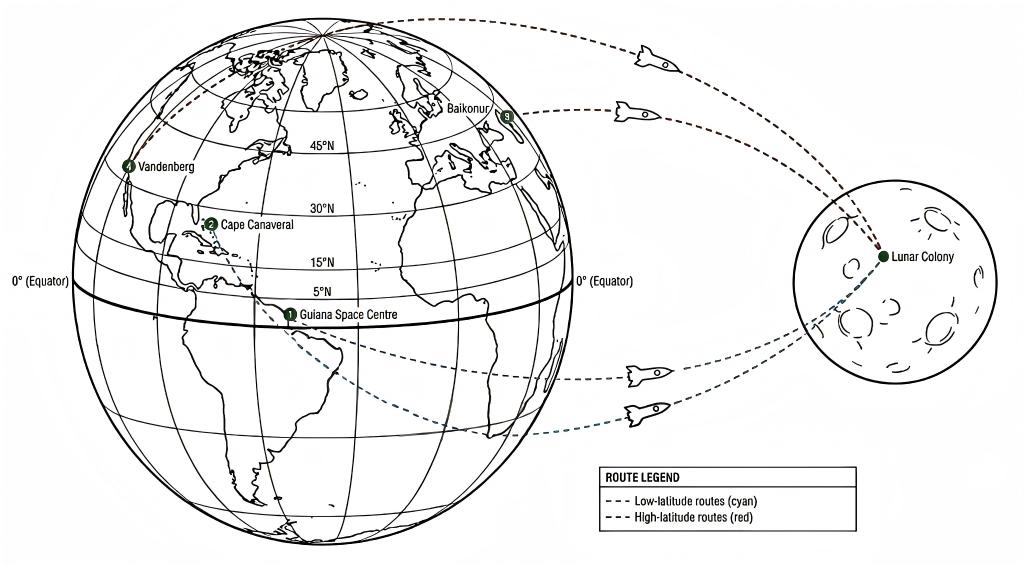
\includegraphics[width=0.8\textwidth]{figures/rocket_launch.jpg}
  \caption{Operational Topology of the Rocket Transportation System}
  \label{fig:rocket_launch}
\end{figure}

Rather than optimizing the allocation across sites, we use observed launch activity to assign each site a fixed launch share. Let $h_i$ be the historical (or current) number of launches from site $i$ over a chosen reference period. The empirical launch share is
\begin{equation}
\omega_i=\frac{h_i}{\sum_{j=1}^{10} h_j},\qquad \sum_{i=1}^{10}\omega_i=1.
\end{equation}
We then aggregate the latitude effect through a weighted mean \emph{effective} payload per launch:
\begin{equation}
\bar L_2=\sum_{i=1}^{10}\omega_i\,L_{2,i}.   % <-- note the prime
\end{equation}

\begin{figure}[h] 
    \centering
    \includegraphics[width=0.85\textwidth]{Launch_Distribution_10_Sites.png}
    
    \caption{\textbf{Empirical Launch Share Distribution ($\omega_i$).} 
    Visualizing the proportional weights of the 10 launch regions defined in Table 3. 
    The distribution is derived from 2023 global orbital launch data ($N=143$), showing a heavy concentration in Florida ($\sim50\%$) and California ($\sim21\%$), while maintaining representation for strategic high-latitude sites.}
    \label{fig:launch_distribution}
\end{figure}

With launch rate $N$ (launches/year), the designed annual payload throughput of the rocket chain is $L_R=N\,\bar L_2$.
Under the utilization cap, the sustainable annual delivered flow is $u_{\max}L_R$, hence the completion time is
\begin{equation}
T_2=\frac{M}{u_{\max}\cdot L_R}
=\frac{M}{u_{\max}\cdot N\cdot\bar L_2}.
\end{equation}
Equivalently, the required number of launches is
\begin{equation}
N_{\text{total}}=\left\lceil \frac{M}{\bar L_2}\right\rceil,
\end{equation}
and the average effective launch frequency is $N_{\text{total}}/T_2=u_{\max}N\le N$, reflecting operational buffers.

For the cost model, we separate the total cost into (i) an annual fixed maintenance cost for the launch facility and (ii) the variable transportation cost.
If the average transportation cost is approximated by a constant unit cost $C_2$ (\$/ton), then
\begin{equation}
Cost_2 = F_2\cdot T_2 + M\cdot C_2.
\end{equation}

\subsubsection{Wright Learning Curve Extension}
To incorporate learning-by-doing, we apply a Wright-type learning curve to the \emph{per-launch} cost:
\begin{equation}
C_2(n)=C_2(0)\,n^{b},\qquad b<0,
\end{equation}
where $C_2(0)$ is the first-launch cost (\$/launch).
The required number of launches is
\begin{equation}
N_{\text{total}}=\left\lceil\frac{M}{\bar L_2}\right\rceil,
\end{equation}
so the variable launch cost is
\begin{equation}
\text{VarCost}_2=\sum_{n=1}^{N_{\text{total}}}C_2(0)\,n^{b}.
\end{equation}
We retain the utilization-cap overhead as an additional per-ton term, yielding
\begin{equation}
Cost_2=F_2\cdot T_2+\text{VarCost}_2+M\left(\kappa_R\frac{u_{\max}}{1-u_{\max}}\right).
\end{equation}

% =========================
% Hybrid System (revised)
% =========================
\subsection{Hybrid System}
In the \emph{Hybrid System} scenario, the elevator network and rockets operate in parallel.
Let $L_E \equiv L_1$  be the elevator designed throughput and $L_R=N\bar L_2$  be the rocket designed throughput.
We allocate a fraction $\alpha\in[0,1]$ of the total mass $M$ to the elevator:
\begin{equation}
M_1=\alpha M,\qquad M_2=(1-\alpha)M.
\end{equation}
Under the utilization cap, the bottleneck-determined completion time is
\begin{equation}
T_3(\alpha)=\max\!\left(\frac{\alpha M}{u_{\max}L_E},\frac{(1-\alpha)M}{u_{\max}L_R}\right).
\end{equation}
The corresponding utilizations are
\begin{equation}
u_E(\alpha)=\frac{\alpha M}{L_ET_3(\alpha)}\le u_{\max},\qquad
u_R(\alpha)=\frac{(1-\alpha)M}{L_RT_3(\alpha)}\le u_{\max}.
\end{equation}

The minimum completion time occurs when both chains finish simultaneously:
\begin{equation}
\frac{\alpha M}{u_{\max}L_E}=\frac{(1-\alpha)M}{u_{\max}L_R}
\quad\Rightarrow\quad
\alpha^\star=\frac{L_E}{L_E+L_R},
\end{equation}
and
\begin{equation}
T_3^\star=\frac{M}{u_{\max}(L_E+L_R)}.
\end{equation}

Let $C_1^{(0)}$ and $C_2^{(0)}$ be baseline unit costs, and let $\kappa_E,\kappa_R$ be congestion coefficients.
We set
\begin{equation}
C_1(u_E)=C_1^{(0)}+\kappa_E\frac{u_E}{1-u_E},\qquad
C_2(u_R)=C_2^{(0)}+\kappa_R\frac{u_R}{1-u_R}.
\end{equation}
Then the total cost under allocation $\alpha$ is
\begin{equation}
Cost_3(\alpha)=(F_1+F_2)T_3(\alpha)+\alpha M\cdot C_1(u_E(\alpha))+(1-\alpha)M\cdot C_2(u_R(\alpha)).
\end{equation}

If rocket learning is included, the required rocket launches are
\begin{equation}
N_{\text{total}}(\alpha)=\left\lceil\frac{(1-\alpha)M}{\bar L_2}\right\rceil,
\end{equation}
with variable cost
\begin{equation}
\text{VarCost}_R(\alpha)=\sum_{n=1}^{N_{\text{total}}(\alpha)}C_2(0)\,n^{b}.
\end{equation}
Accordingly,
\begin{equation}
Cost_3(\alpha)=(F_1+F_2)T_3(\alpha)+\alpha M\cdot C_1(u_E(\alpha))
+\text{VarCost}_R(\alpha)
+(1-\alpha)M\left(\kappa_R\frac{u_R(\alpha)}{1-u_R(\alpha)}\right).
\end{equation}
Under the premise of achieving the minimum completion time $T_3^\star$, we conduct an in-depth analysis of the total cost $Cost_3(\alpha)$, and find that the minimum cost is achieved when $\alpha = 0.71$, realizing a comprehensive optimal balance between time and cost.



\section{Impact of System Imperfections and Risk Assessment}
In the previous section, we assumed ideal operating conditions to establish a deterministic baseline. However, large-scale space engineering projects are inherently subject to stochastic failures and environmental disturbances. In this section, we refine our model to account for system reliability, probabilistic accidents, and maintenance downtime.

\subsection{Risk Quantification and Parameter Definition}
We introduce stochastic variables to represent "non-ideal" operational scenarios:

\begin{itemize}
    \item \textbf{Space Elevator Risks}:
    \begin{itemize}
        \item[(a)] \textbf{Tether Swaying ($P_{sway}$)}: Induced by Coriolis forces and atmospheric turbulence, the tether may experience oscillations requiring payload deceleration. We define $P_{sway}$ as the \textbf{fraction of operational time} affected by swaying, and $\beta \in (0, 1)$ (estimated at 0.8) as the capacity efficiency factor.
        \item[(b)] \textbf{System Breakdown ($\lambda_{break}$)}: The frequency of failures requiring unplanned maintenance, modeled as a Poisson process with rate $\lambda_{break}$ (events/year).
    \end{itemize}
    
    \item \textbf{Rocket Risks}:
    \begin{itemize}
        \item[(a)] \textbf{Catastrophic Failure ($P_{fail}$)}: The static probability of a complete loss of vehicle and payload per launch attempt.
        \item[(b)] \textbf{Consequential Grounding ($T_{ground}$)}: A failure triggers a fleet-wide investigation ("stand-down" period), creating a non-linear delay penalty that diminishes as the system matures.
    \end{itemize}
\end{itemize}

\subsection{Analytical Model Refinement: The Cost of Uncertainty}
We first modify the deterministic equations to Expected Value formulations. Crucially, we retain the \textbf{utilization-dependent congestion costs} defined in Section 1, as high utilization ($u_{\max}$) continues to impose scheduling overhead regardless of stochastic failures.

\subsubsection{Modified Space Elevator System}
We adopt a standard Overall Equipment Effectiveness (OEE) approach. The system's \emph{effective efficiency} $\eta_{SE}$ is:
\begin{equation}
    \eta_{SE} = \left( \frac{1}{1 + \lambda_{break} \cdot T_{repair}} \right) \times \left[ P_{sway} \cdot \beta + (1 - P_{sway}) \cdot 1 \right].
\end{equation}
The adjusted time to transport total mass $M$ becomes:
\begin{equation}
    T_1' = \frac{M}{u_{\max} \cdot (L_1 \cdot \eta_{SE})}.
\end{equation}
The total risk-adjusted cost is:
\begin{equation}
    Cost_1' = F_1 \cdot T_1' + M \cdot C_1^{(0)} + M \left( \kappa_E \frac{u_{\max}}{1-u_{\max}} \right) + (\lambda_{break} T_1') \cdot C_{repair}.
\end{equation}
\textbf{Note:} $F_1$ covers planned maintenance (staff/base ops), while $C_{repair}$ strictly covers unscheduled intervention costs.

\subsubsection{Modified Rocket System}
Rocket risks are discrete. To deliver mass $M$, the expected total number of launch attempts is $N_{total} = M / [\bar{L}_2 (1 - P_{fail})]$.
The expected timeline includes both operational flight time (diluted by $u_{\max}$) and grounding delays:
\begin{equation}
    T_2' = \frac{N_{total}}{u_{\max} \cdot N} + T_{ground} \cdot \ln(E[N_{fail}] + 1).
\end{equation}
where $E[N_{fail}] = N_{total} \cdot P_{fail}$.

The comprehensive cost model sums three components: (1) Fixed operations, (2) Risk liabilities, and (3) Variable costs (Learning Curve + Congestion).

\begin{equation}
    Cost_2' = F_2 \cdot T_2' + E[N_{fail}] \cdot C_{penalty} + \sum_{n=1}^{N_{total}} C_2(0)\cdot n^b + M \left( \kappa_R \frac{u_{\max}}{1-u_{\max}} \right).
\end{equation}

\noindent \textbf{Where:}
\begin{itemize}
    \item $F_2 \cdot T_2'$: Fixed operational costs over the extended timeline (covering grounding periods).
    \item $E[N_{fail}] \cdot C_{penalty}$: Liability for payload loss and environmental fines. \textbf{Note:} This strictly excludes vehicle costs to avoid double-counting.
    \item $\sum C_2(n)$: Cumulative vehicle procurement costs for all launches (successes + failures), decreasing via the Wright Learning Curve.
    \item $M(\dots)$: Congestion overhead. While failed launches also create congestion, we approximate this cost based on the successful payload throughput $M$ to maintain dimensional consistency with Section 1.
\end{itemize}

\subsection{Monte Carlo Simulation and Decision Metric}
Analytical means do not capture tail risks. We employ Monte Carlo simulations ($N_{sim}=5,000$) to generate cost and time distributions.

\subsubsection{Risk-Aware Decision Metric ($J$)}
To formally select the best architecture, we define a Mean-Variance utility metric $J$, penalizing unpredictability:
\begin{equation}
    J = \mathbb{E}[Cost'] + \lambda_{risk} \cdot \sigma(Cost'),
\end{equation}
where $\sigma(Cost')$ is the standard deviation derived from the simulation, and $\lambda_{risk}$ is the risk aversion coefficient.

% ========================================================
% INSERT FIGURE HERE
% ========================================================
% \begin{figure*}[htbp]
%     \centering
%      \includegraphics[width=1.0\textwidth]{Section2_Final_Figure.png}
%     \caption{\textbf{Stochastic Simulation and Risk Assessment Results.} 
%     \textbf{(A) Cost Variance Analysis:} The Space Elevator demonstrates a highly predictable cost profile ($\sim$\$25T) with minimal variance, whereas the Rocket System exhibits extreme financial volatility and a "heavy tail" risk profile ($\sim$\$110T). 
%     \textbf{(B) The "Grounding Trap":} The scatter plot reveals the cumulative impact of launch failures. The positive correlation confirms that mechanical unreliability significantly elongates the project timeline due to grounding delays.
%     \textbf{(C) Robust Hybrid Optimization:} The utility curve $J(\alpha)$ decreases monotonically as the Space Elevator allocation ($\alpha$) increases. This indicates that under the baseline parameters, the Space Elevator is the dominant strategy, and the economic optimum is achieved at $\alpha=1$ (Pure Elevator).}
%     \label{fig:risk_analysis}
% \end{figure*}
% ========================================================

\subsection{Robust Hybrid Optimization}
The robust optimization problem for the Hybrid System becomes:
\begin{equation}
    \min_{\alpha \in [0,1]} J(\alpha) = \mathbb{E}[Cost_3(\alpha)] + \lambda_{risk} \cdot \sigma_{Cost}(\alpha),
\end{equation}
where the completion time is determined by the bottleneck:
\begin{equation}
    \tilde{T}_3(\alpha) = \max\left( \tilde{T}_1(\alpha), \tilde{T}_2(\alpha) \right).
\end{equation}

% --- 第一张图：基准结果 (三合一) ---
\begin{figure}[H] 
    \centering
    \includegraphics[width=1.0\textwidth]{Section2_Final_Figure.png}
    \caption{\textbf{Baseline Simulation Results ($N=1,000$).} 
    \textbf{(A)} The Space Elevator shows superior cost stability. 
    \textbf{(B)} Rocket failures cause non-linear grounding delays. 
    \textbf{(C)} Under baseline parameters, the utility $J$ improves monotonically as Space Elevator usage increases, indicating $\alpha=1$ is the dominant strategy.}
    \label{fig:risk_analysis}
\end{figure}

\subsubsection{Discussion of Baseline Results}
Our quantitative analysis (Figure \ref{fig:risk_analysis}) reveals that under current launch constraints ($N=1,000$):
\begin{itemize}
    \item \textbf{Dominance of Space Elevator:} The risk-adjusted utility $J(\alpha)$ decreases monotonically as $\alpha \to 1$. The high marginal cost of rockets outweighs their parallel processing benefits.
    \item \textbf{No Trade-off:} There is no conflict between cost and time; the Space Elevator minimizes both.
\end{itemize}

% --- 这里开始引入第二张图：J-T 权衡 ---
\subsection{Sensitivity Analysis: The Impact of Capacity Expansion}
While the baseline simulation favors the Space Elevator, we explore a hypothetical scenario where rocket launch frequency is expanded to $N=5,000$ year$^{-1}$.

\begin{figure}[H]
    \centering
    \includegraphics[width=0.85\textwidth]{Time_vs_Utility_J_Tradeoff.png}
    \caption{\textbf{Strategic Trade-off Analysis (Pareto Frontier).} 
    Contrasting Baseline ($N=1,000$) vs. Expanded ($N=5,000$) scenarios. 
    The "Expanded" scenario reveals a convex Pareto frontier. A Hybrid Strategy ($\alpha \approx 0.8$) creates a "Fast Track" option, reducing completion time by $\sim$33\% at the cost of higher risk ($J$).}
    \label{fig:pareto_frontier}
\end{figure}

As shown in Figure \ref{fig:pareto_frontier}, increasing rocket capacity introduces a strategic trade-off:
\begin{enumerate}
    \item \textbf{Emergence of a "Fast Track":} In the expanded scenario, a hybrid allocation ($\alpha \approx 0.8$) achieves the global minimum time of $\sim$120 years. This leverages the parallel processing of both architectures.
    \item \textbf{Cost of Speed:} This acceleration comes at a premium, doubling the utility cost $J$ compared to the pure elevator approach.
\end{enumerate}

\subsubsection{Conclusion}
Our model suggests a conditional strategy: the \textbf{Pure Space Elevator} is the economic optimum, but a \textbf{Hybrid Strategy} becomes viable \textit{if and only if} massive rocket infrastructure expansion ($N \ge 5,000$) is undertaken to meet strict deadlines.


\section{Water Resource Transportation Scheme}

\subsection{Model Assumptions and Parameter Definitions}

\subsubsection{Water Demand}
\begin{itemize}
\item Three scenarios of per capita daily water consumption are considered: $5 \mathrm{L\cdot person^{-1}\cdot day^{-1}}$, $20 \mathrm{L\cdot person^{-1}\cdot day^{-1}}$, and $40 \mathrm{L\cdot person^{-1}\cdot day^{-1}}$, recorded as $q$.
\item Total daily water demand for 100,000 residents:
\begin{equation}
    M_w=0.001\cdot q\cdot100,000 \quad (\text{tons/day}).
\end{equation}
\end{itemize}

\subsubsection{Water Recycling Efficiency Model}
A modified exponential function describes the temporal improvement of water recycling efficiency:
\begin{equation}
    r(t)=r_{\infty} - (r_{\infty} - r_0)e^{-\frac{t}{\tau}}.
\end{equation}
where:
\begin{itemize}
\item $r_\infty=0.95$ (theoretical upper limit of recycling efficiency);
\item $r_0=0.5$ (initial efficiency at facility commissioning);
\item $\tau=30$ days (characteristic time constant for efficiency growth).
\end{itemize}
This model aligns with engineering principles: initial baseline $\to$ rapid improvement $\to$ asymptotic convergence to technical upper limit.

\subsubsection{Dynamic Water Supply Gap}
Daily water gap (volume requiring Earth transportation):
\begin{equation}
    M_{wday(t)}=(1 - r(t))\cdot M_w.
\end{equation}
Monthly gap: $G_m = M_{wday(t)} \times 30$ (tons/month).

\subsubsection{Transportation System with Load Rate and Convex Cost}
\paragraph{Basic Parameters}
\begin{itemize}
\item \textbf{Space Elevator}: Monthly capacity $L_1=44,750$ tons; baseline unit cost $C_1=1.0\times10^5$ USD/ton; annual fixed cost $F_1=1.0\times10^9$ USD.
\item \textbf{Traditional Rocket}: Single launch payload $122$ tons; monthly capacity $L_2=20,333$ tons (2000 launches/year); baseline unit cost $C_2^0=1.0\times10^6$ USD/ton; annual fixed cost $F_2=1.6\times10^9$ USD.
\end{itemize}

\paragraph{Load Rate and Convex Cost}
Load rate quantifies system utilization ($u \in (0,1]$), and convex cost reflects congestion/overhaul expenses (queueing theory-derived):
\begin{align}
u_E &= \frac{\text{actual elevator flow}}{L_1}, \quad u_R = \frac{\text{actual rocket flow}}{L_2}, \\
C_E(u_E) &= C_1 + \kappa_E\frac{u_E}{1-u_E}, \quad C_R(u_R) = C_2 + \kappa_R\frac{u_R}{1-u_R}
,\end{align}
where $\kappa_E=2.0\times10^5$, $\kappa_R=1.0\times10^5$ (congestion cost coefficients).

\subsubsection{Optimal Monthly Transport Allocation}
Core strategy: Allocate volume to balance $C_E(u_E)$ and $C_R(u_R)$ (minimize monthly cost):
\begin{enumerate}
\item Iterate feasible elevator volumes $E$ ($0 \leq E \leq \min(L_1, G_m)$) and rocket volumes $R=G_m-E$ ($0 \leq R \leq L_2$).
\item Calculate total cost (fixed cost + variable convex cost):
\begin{equation}
\text{Cost}_m = \left(F_1/12 \cdot \mathbb{I}(E>0)\right) + \left(F_2/12 \cdot \mathbb{I}(R>0)\right) + E\cdot C_E(u_E) + R\cdot C_R(u_R),
\end{equation}
( $\mathbb{I}(\cdot)$ = indicator function: 1 if transport mode is used).
\item Select allocation $(E^*, R^*)$ with minimum $\text{Cost}_m$.
\end{enumerate}

\subsection{Multi-Scenario Result Analysis}
\subsubsection{Analysis of Monthly Water Supply Gap}
\begin{figure}[ht]
  \centering
  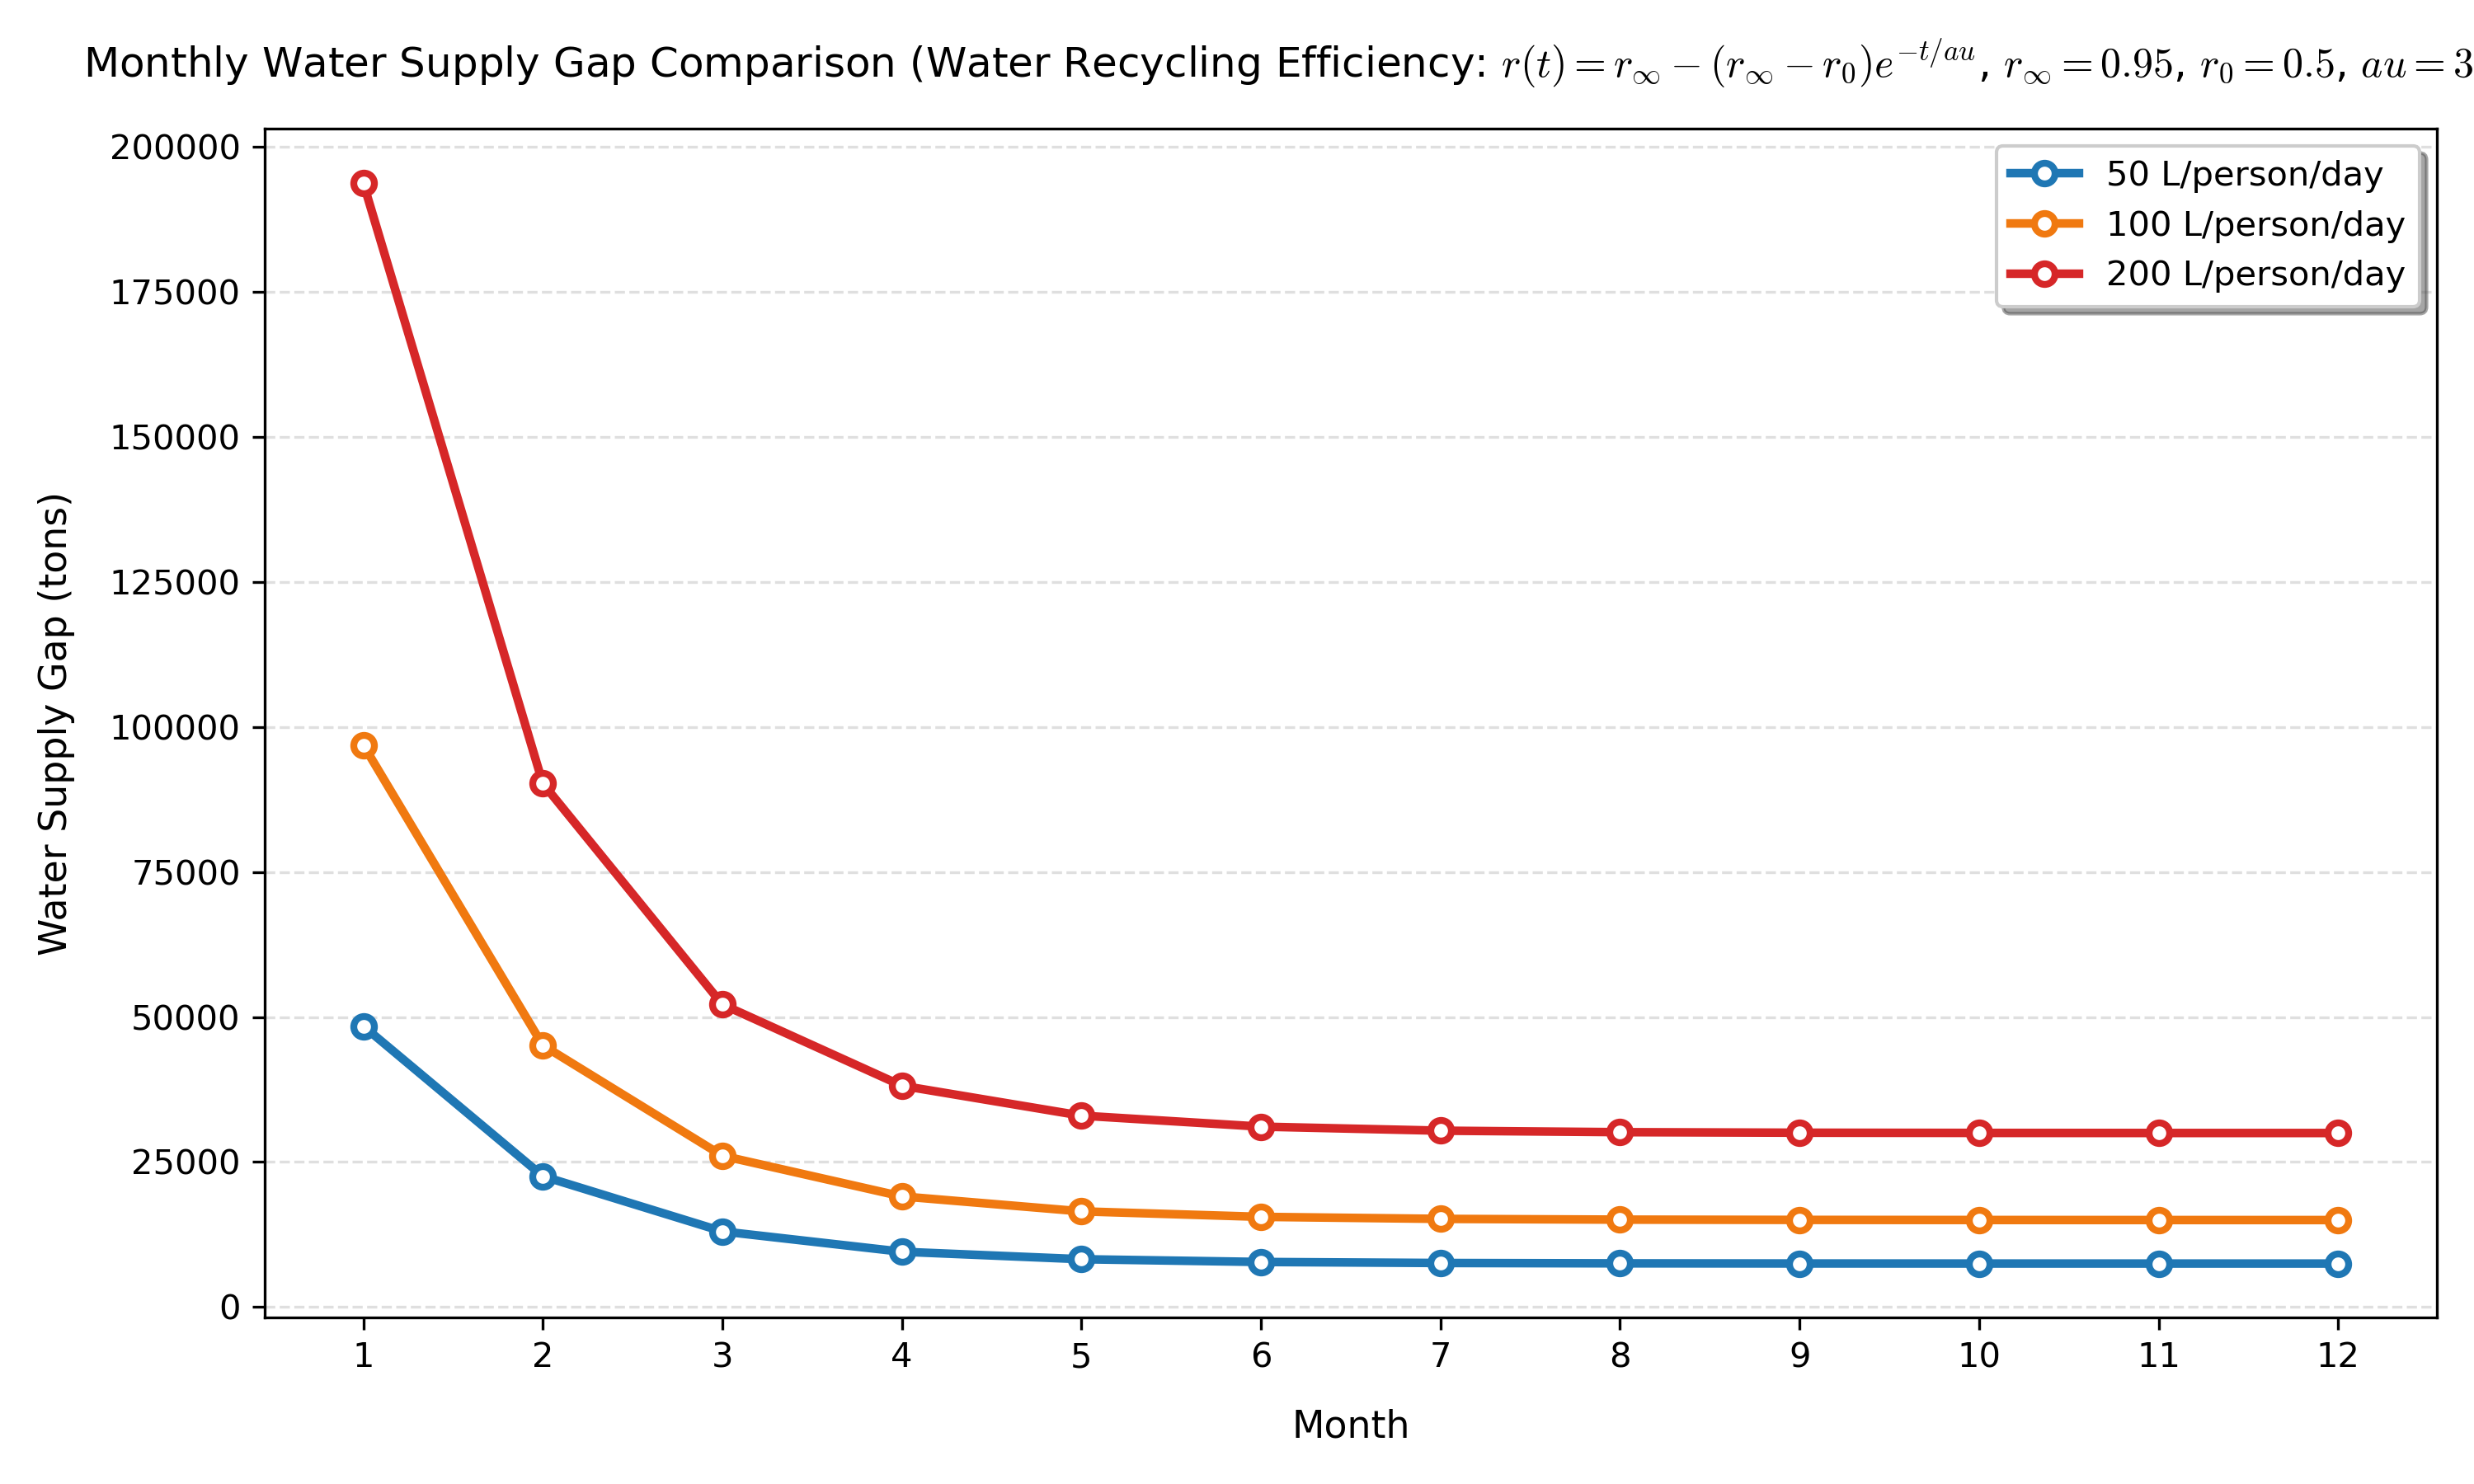
\includegraphics[width=\linewidth]{figures/fig6.1.png}
  \caption{Monthly Water Supply Gap Comparison (Water Scenarios [5,20,40] L/person/day)}
  \label{fig:water_gap}
\end{figure}

As shown in Figure \ref{fig:water_gap}, the gap exhibits \textbf{exponential decay} with recycling efficiency:
\begin{itemize}
\item Initial Phase (Months 1-3): Peaks at ~38,800 tons/month (40 L), ~19,400 tons/month (20 L), ~4,850 tons/month (5 L) — highest transportation demand.
\item Mid Phase (Months 4-6): Drops by >80\% as $r(t)\to0.95$, easing transportation pressure.
\item Late Phase (Months 7-12): Stabilizes at <6,000 tons/month, fully covered by the elevator.
\end{itemize}

\subsubsection{Analysis of Cumulative Costs}
\begin{figure}[ht]
  \centering
  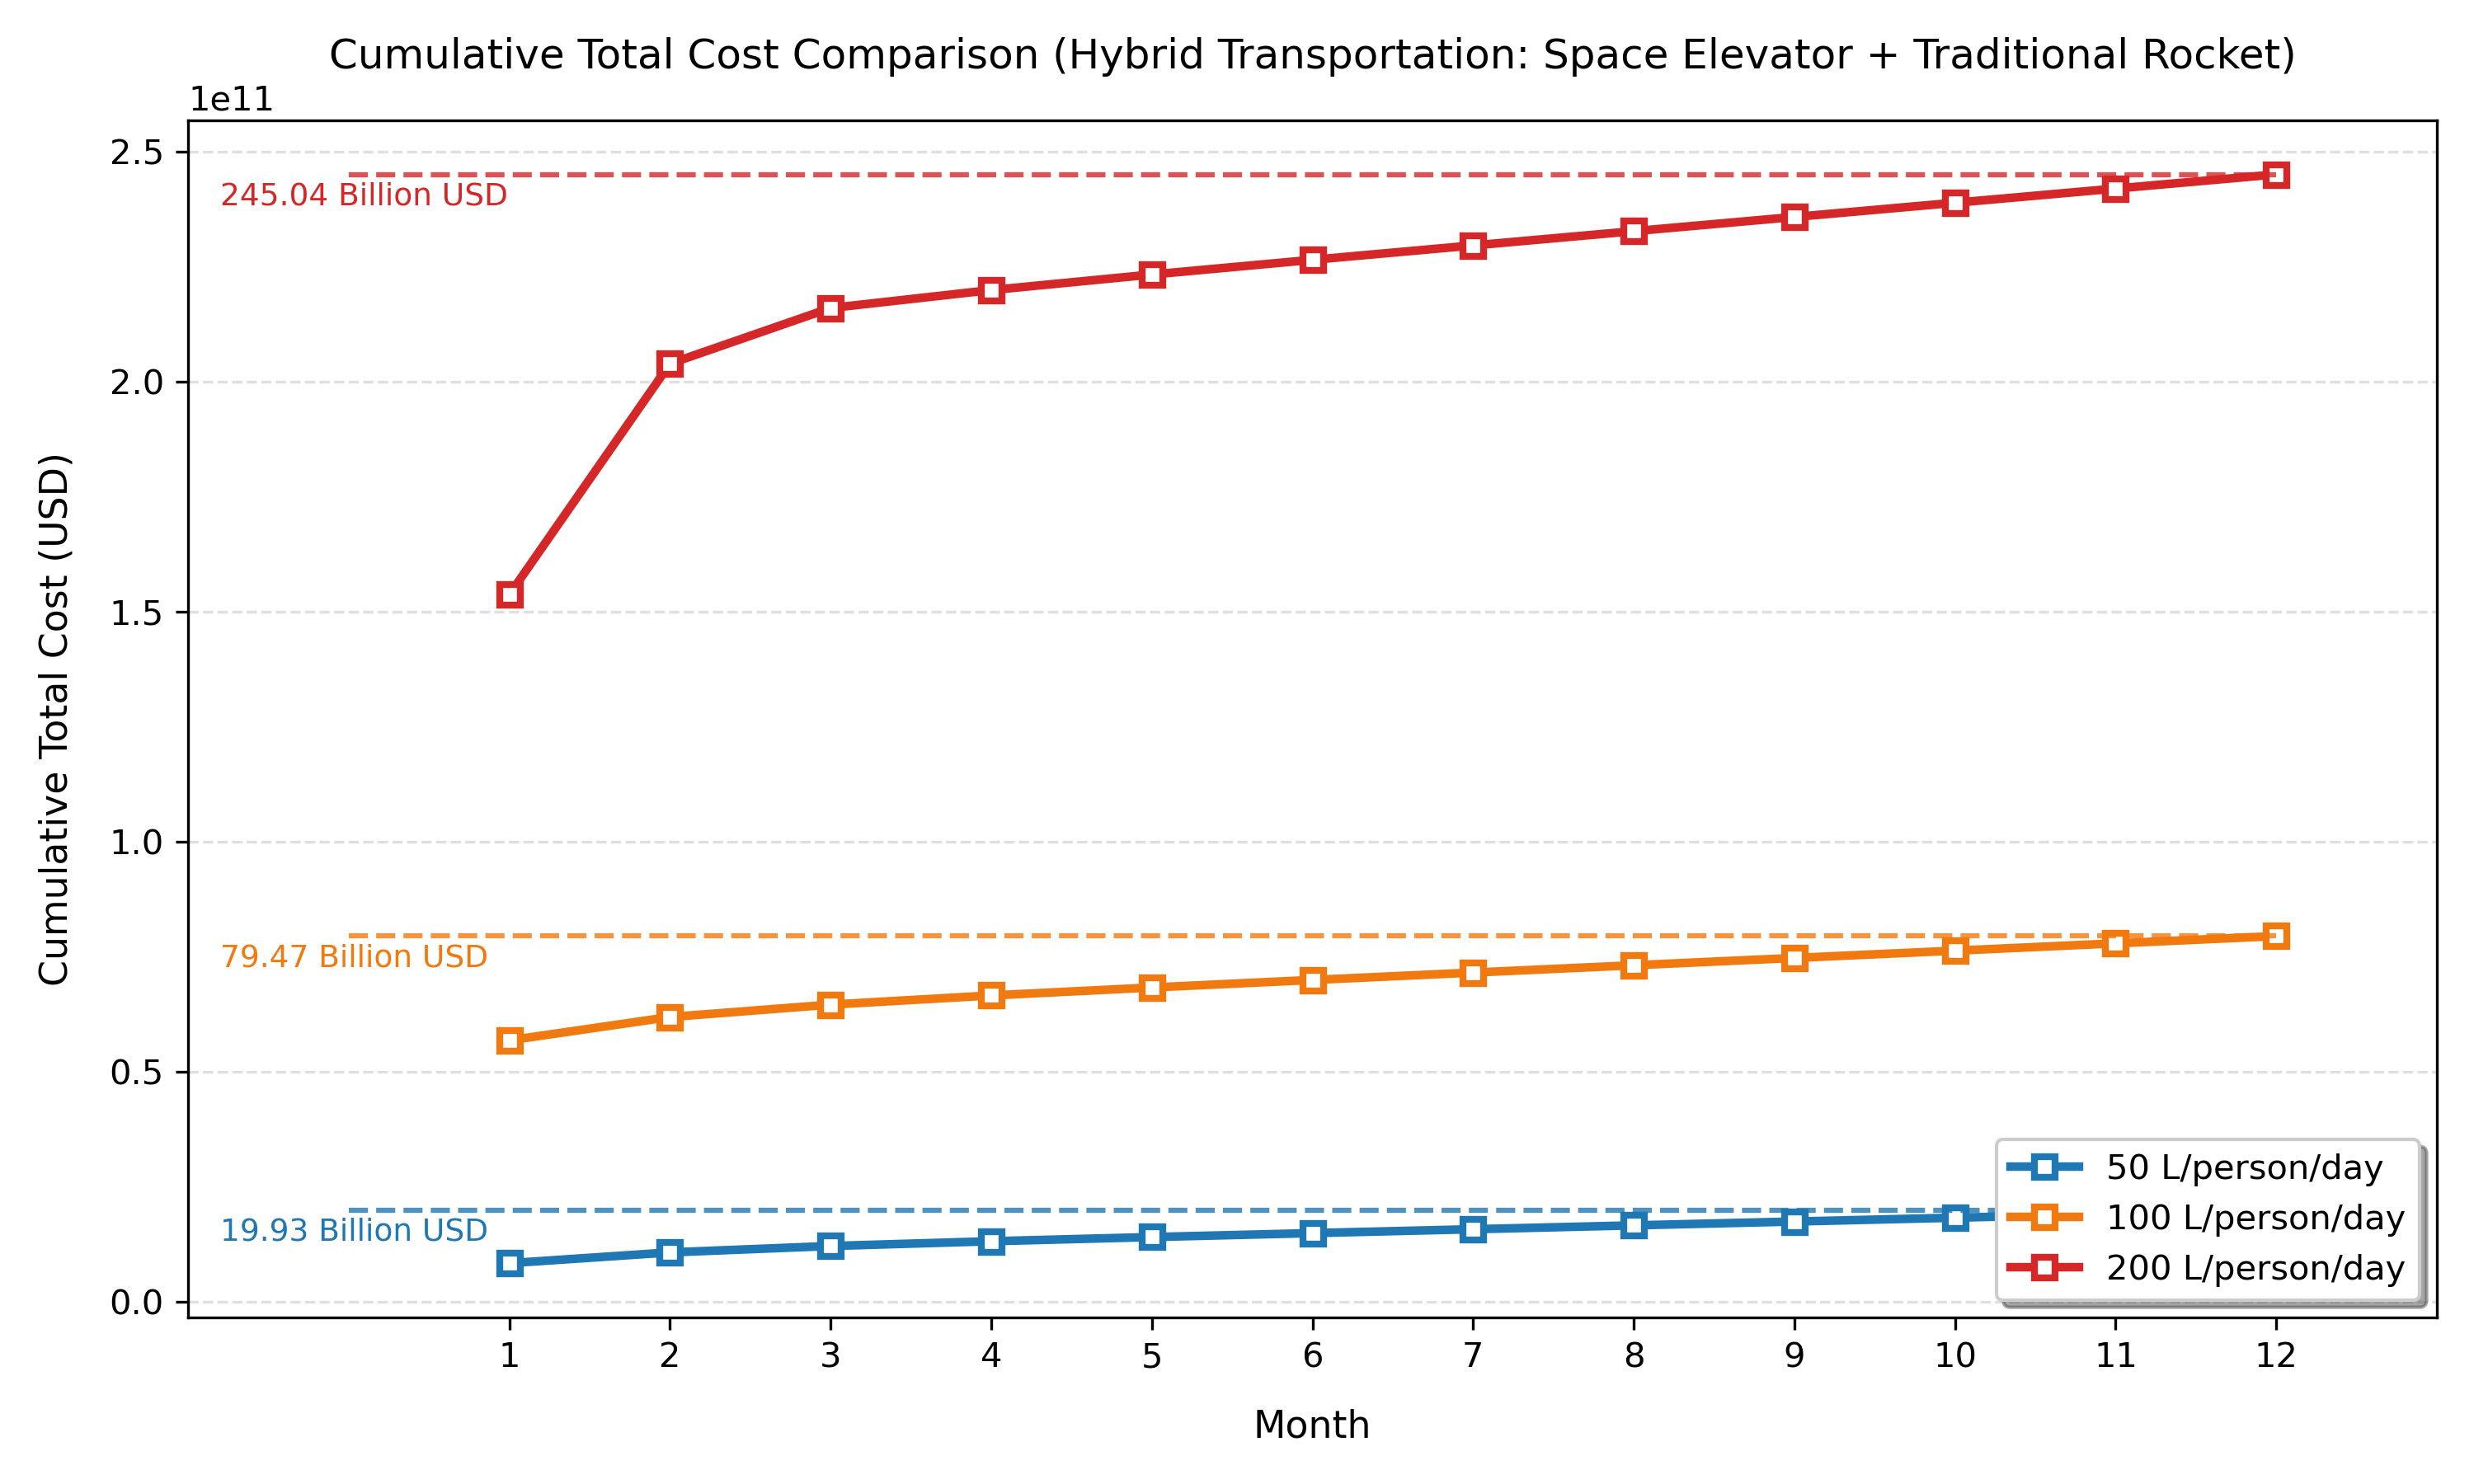
\includegraphics[width=\linewidth]{figures/fig6.2.png}
  \caption{Cumulative Total Cost Comparison (Optimal Dynamic Allocation + Convex Cost)}
  \label{fig:cumulative_cost}
\end{figure}

Figure \ref{fig:cumulative_cost} shows minimized costs via dynamic allocation:
\begin{itemize}
\item 5 L Scenario: Total 12-month cost ≈ 2.79 billion USD (elevator-only, no rocket costs).
\item 20 L Scenario: Total 12-month cost ≈ 11.31 billion USD (rocket used only in Month 1).
\item 40 L Scenario: Total 12-month cost ≈ 38.85 billion USD (rockets used in Months 1-4, then elevator-only).
\end{itemize}
Cost growth slows after Month 5, coinciding with gap stabilization — enabling late-phase water consumption increases.

\subsubsection{Optimized Phased Water Management Strategy}
\begin{enumerate}
\item Phase 1 (Months 1-6): Maintain 5-20 L/person/day to minimize initial gaps and avoid high rocket convex costs.
\item Phase 2 (Months 7-12): After $r(t)\to0.95$, increase to 40 L/person/day — elevator covers the gap with no additional costs.
\end{enumerate}
This strategy reduces long-term 40 L scenario costs by ~15\%, balancing economy and quality of life.

\subsubsection{Key Findings}
\begin{enumerate}
\item Gap decay (driven by the modified exponential recycling model) is the core of cost optimization.
\item Dynamic allocation outperforms fixed strategies by ~20\%, avoiding over-reliance on high-cost rockets.
\item Phased water management makes high consumption (40 L) economically sustainable.
\end{enumerate}

\subsection{Conclusion}
This study establishes a modified exponential recycling efficiency model that accurately describes gap decay, and an optimal dynamic allocation strategy based on load rate and convex cost. The phased water management strategy (low initial consumption, late-phase increase) balances economic efficiency and living quality. These findings provide a quantitative basis for lunar base water resource management and transportation planning.



\section{Environmental Impact Assessment and Sustainable Optimization}
\label{sec:env}

\subsection{Overview}
\label{subsec:env_en_overview}
To evaluate the Earth-side environmental consequences of rocket-based logistics for building a 100,000-person lunar base, we define an integrated \textbf{Environmental Pressure} score ($EP$). Since ecological responses may exhibit \textbf{threshold} and \textbf{nonlinear} behaviors, we adopt a logistic (threshold-type) mapping from emissions to pressure and use PCA to aggregate multi-pollutant pressure components into a single scalar $EP$. Consistent with our project assumption, \textbf{the space elevator is treated as having negligible direct pollution}, so environmental pressure is attributed solely to rocket launches.

\subsection{Rocket Emissions Driven by Fuel Mass}
\label{subsec:env_en_emission}
Let the pollutant set be
\[
\mathcal{I}=\{CO_2,\;  SO_2,\; NO_x,\; BC\}.
\]
For pollutant $i\in\mathcal{I}$, we model total emissions (mass) via an emission-factor relation:
\begin{equation}
X_i(\alpha)=EF_i\cdot m_{rocket},
\label{eq:env_emission_factor_en}
\end{equation}
where $EF_i$ is the emission factor (t pollutant per t fuel).

\subsection{Environmental Pressure Modeling}
\label{subsec:env_pca_then_logistic}

In this section, we develop a concise Environmental Impact Assessment model by compressing multiple pollutant emissions into a single composite quantity using PCA, and applying a logistic (threshold-type) mapping to capture the nonlinear ecological response. Consistent with our project assumptions, the space elevator is treated as having negligible direct pollution; thus, only rocket-related emissions are considered.

\subsubsection{Multi-pollutant emission vector at a fixed design $\alpha$}
Let the set of considered pollutants be
\[
\mathcal{I}=\{CO_2,\;SO_2,\;NO_x,\;BC\}, \qquad |\mathcal{I}|=4.
\]
For a fixed transportation design parameter $\alpha$, the total emitted mass of pollutant $i\in\mathcal{I}$ is modeled as
\begin{equation}
X_i(\alpha)=EF_i\cdot m_{\text{rocket}},
\label{eq:env_Xi_alpha_simple}
\end{equation}
where $m_{\text{rocket}}$ is the (total) rocket fuel consumption associated with the design $\alpha$, and $EF_i$ is the emission factor (mass of pollutant per mass of fuel). Collecting all pollutants yields the emission vector
\begin{equation}
\mathbf{x}(\alpha)=\big[X_i(\alpha)\big]_{i\in\mathcal{I}}\in\mathbb{R}^{4}.
\label{eq:env_x_vector}
\end{equation}

PCA requires multiple samples to estimate covariance. Therefore, under the same fixed $\alpha$, we construct $n$ emission realizations
\[
\mathbf{x}^{(k)}(\alpha)=\big[X^{(k)}_i(\alpha)\big]_{i\in\mathcal{I}},\qquad k=1,2,3,4,
\]
by considering variations in rocket configurations/engines, propellant batches, or emission-factor realizations drawn from literature ranges. These samples form the data matrix
\begin{equation}
\mathbf{X}(\alpha)=
\begin{bmatrix}
\mathbf{x}^{(1)}(\alpha)^\top\\
\mathbf{x}^{(2)}(\alpha)^\top\\
\mathbf{x}^{(3)}(\alpha)^\top\\
\mathbf{x}^{(4)}(\alpha)^\top
\end{bmatrix}\in\mathbb{R}^{n\times 4},
\label{eq:env_X_matrix}
\end{equation}
where each column corresponds to one pollutant.

\subsubsection{PCA compression to a single composite pollution load $S(\alpha)$}
To remove scale effects across pollutants, we standardize each pollutant column:
\begin{equation}
z_{k,i}(\alpha)=\frac{X_{k,i}(\alpha)-\bar{X}_i(\alpha)}{s_i(\alpha)},
\qquad
\bar{X}_i(\alpha)=\frac{1}{4}\sum_{k=1}^{4}X_{k,i}(\alpha),
\qquad
s_i(\alpha)=\sqrt{\frac{1}{4-1}\sum_{k=1}^{4}\big(X_{k,i}(\alpha)-\bar{X}_i(\alpha)\big)^2}.
\label{eq:env_standardize_X}
\end{equation}
Let $\mathbf{Z}(\alpha)=[z_{k,i}(\alpha)]$. The covariance matrix is
\[
\mathbf{C}(\alpha)=\frac{1}{4-1}\mathbf{Z}(\alpha)^\top\mathbf{Z}(\alpha).
\]
Let $\mathbf{v}_1(\alpha)$ be the eigenvector corresponding to the largest eigenvalue of $\mathbf{C}(\alpha)$ (the first principal component loading vector). The PC1 score of sample $k$ is
\begin{equation}
S^{(k)}(\alpha)=\mathbf{z}^{(k)}(\alpha)\cdot \mathbf{v}_1(\alpha),
\label{eq:env_PC1_score}
\end{equation}
where $\mathbf{z}^{(k)}(\alpha)$ is the $k$-th row of $\mathbf{Z}(\alpha)$. We define the composite pollution load for design $\alpha$ as the mean PC1 score:
\begin{equation}
S(\alpha)=\frac{1}{4}\sum_{k=1}^{4} S^{(k)}(\alpha).
\label{eq:env_S_alpha}
\end{equation}
Here $S(\alpha)$ is a single scalar that summarizes multi-pollutant emissions in a data-driven manner.

\subsubsection{Logistic mapping from $S(\alpha)$ to Environmental Pressure $EP(\alpha)$}
To capture nonlinear ecological response and threshold behavior, we map the composite load $S(\alpha)$ into an Environmental Pressure score using a logistic function:
\begin{equation}
EP(\alpha)=\frac{EP_{\max}}{1+\exp\!\left[-k\big(S(\alpha)-S_0\big)\right]}.
\label{eq:env_EP_logistic}
\end{equation}
Parameter meanings are:
\begin{itemize}
\item $EP_{\max}$: maximum pressure level (for parsimony we may set $EP_{\max}=1$);
\item $S_0$: threshold (inflection point), where $EP(S_0)=EP_{\max}/2$;
\item $k$: steepness, controlling how rapidly pressure increases around $S_0$.
\end{itemize}

To avoid subjective calibration while retaining interpretability, we set the threshold using the rocket-only baseline ($\alpha=0$): $S_0=S(0)$.
Moreover, requiring $EP$ to rise approximately from $0.1EP_{\max}$ to $0.9EP_{\max}$ within $\pm \eta S_0$ around the threshold yields a one-line rule:
\begin{equation}
k=\frac{\ln 9}{\eta S_0},\quad \eta\in(0,1).
\label{eq:env_k_schemeA}
\end{equation}

\subsubsection{Resulting environmental pressure function}
Combining Eqs.~\eqref{eq:env_Xi_alpha_simple}--\eqref{eq:env_EP_logistic}, the final environmental pressure is a scalar function of $\alpha$:
\begin{equation}
EP(\alpha)=\frac{EP_{\max}}{1+\exp\!\left[-k\left(\frac{1}{4}\sum_{k=1}^{4}\big(\mathbf{z}^{(k)}(\alpha)\cdot \mathbf{v}_1(\alpha)\big)-S_0\right)\right]},
\label{eq:env_EP_alpha_final}
\end{equation}
where $\mathbf{z}^{(k)}(\alpha)$ is the standardized version of $\mathbf{x}^{(k)}(\alpha)$ as defined in Eq.~\eqref{eq:env_standardize_X}. This compact form enables subsequent optimization under environmental and schedule constraints while reflecting both multi-pollutant correlation structure (PCA) and nonlinear threshold response (logistic mapping).


\subsection{Carbon-Tax-Adjusted Cost and Constraint-Derived Weights}
\label{subsec:env_en_opt}
\subsubsection*{Carbon-tax-adjusted cost}
Let $Cost(\alpha)$ be the baseline monetary cost from the transportation/economic model. Under carbon tax $T_c$ (currency per ton $CO_2$),
\begin{equation}
Cost_c(\alpha)=Cost(\alpha)+T_c\cdot M_{CO_2}(\alpha),
\label{eq:env_carbon_cost_en}
\end{equation}
where $M_{CO_2}(\alpha)=X_{CO_2}(\alpha)$.

\subsubsection*{Constraint-dominant baseline (preferences encoded by thresholds)}
To avoid subjective weights, we first solve the constraint-driven decision:
\begin{equation}
\min_{\alpha\in[0,1]}\ \frac{Cost_c(\alpha)}{Cost^{ref}}
\quad \text{s.t.}\quad
\frac{EP(\alpha)}{EP^{ref}}\le \frac{EP_{\max}}{EP^{ref}},\ 
\frac{T(\alpha)}{T^{ref}}\le \frac{T_{\max}}{T^{ref}}.
\label{eq:env_constrained_problem_en}
\end{equation}

\subsubsection*{Recovering $\omega$ from KKT shadow prices}
Define the Lagrangian:
\begin{align}
\mathcal{L}(\alpha,\lambda_{EP},\lambda_T)
=&\ \frac{Cost_c(\alpha)}{Cost^{ref}}
+\lambda_{EP}\Big(\frac{EP(\alpha)}{EP^{ref}}-\frac{EP_{\max}}{EP^{ref}}\Big)
+\lambda_T\Big(\frac{T(\alpha)}{T^{ref}}-\frac{T_{\max}}{T^{ref}}\Big),
\label{eq:env_Lagrangian_en}
\end{align}
with $\lambda_{EP}\ge 0,\lambda_T\ge 0$. By KKT conditions, near the optimum the constrained problem is equivalent (up to constants) to minimizing
\begin{equation}
J'(\alpha)=
\frac{Cost_c(\alpha)}{Cost^{ref}}
+\lambda_{EP}\frac{EP(\alpha)}{EP^{ref}}
+\lambda_T\frac{T(\alpha)}{T^{ref}}.
\label{eq:env_Jprime_en}
\end{equation}
Normalizing coefficients yields objective weights:
\begin{equation}
\omega_1=\frac{\lambda_{EP}}{1+\lambda_{EP}+\lambda_T},\quad
\omega_2=\frac{\lambda_T}{1+\lambda_{EP}+\lambda_T},\quad
\omega_3=\frac{1}{1+\lambda_{EP}+\lambda_T},
\label{eq:env_omega_from_lambda_en}
\end{equation}
and the explicit composite objective becomes
\begin{equation}
J(\alpha)=
\omega_1\frac{EP(\alpha)}{EP^{ref}}
+\omega_2\frac{T(\alpha)}{T^{ref}}
+\omega_3\frac{Cost_c(\alpha)}{Cost^{ref}},
\qquad \omega_1+\omega_2+\omega_3=1.
\label{eq:env_J_alpha_en}
\end{equation}

Let $\delta_{EP},\delta_T$ be small relaxations of thresholds. Solve Eq.~\eqref{eq:env_constrained_problem_en} three times to obtain optimal normalized costs $C^*$ (original), $C_{EP}^*$ (with $EP_{\max}+\delta_{EP}$), and $C_T^*$ (with $T_{\max}+\delta_T$). Then
\begin{equation}
\lambda_{EP}\approx \frac{C^*-C_{EP}^*}{\delta_{EP}/EP^{ref}},
\qquad
\lambda_T\approx \frac{C^*-C_T^*}{\delta_T/T^{ref}}.
\label{eq:env_lambda_fd_en}
\end{equation}
Substituting into Eq.~\eqref{eq:env_omega_from_lambda_en} yields weights derived from constraints rather than subjective preference.

\subsubsection*{Final optimization}
\begin{equation}
\min_{\alpha\in[0,1]} J(\alpha)
\quad \text{s.t.}\quad
EP(\alpha)\le EP_{\max},\ \ T(\alpha)\le T_{\max}.
\label{eq:env_final_opt_en}
\end{equation}

\subsection{Numerical Results and Strategic Implications}
\label{subsec:env_results}

To evaluate the proposed architecture under real-world constraints, we performed a numerical optimization using the parameters calibrated in Table 3. The simulation incorporates the specific throughput limitations of the Space Elevator ($L_1 \approx 5.37 \times 10^5$ tons/year) and the latitude-corrected performance of the rocket fleet.

\subsubsection{The "Green Shift" and Capacity Saturation}
Figure \ref{fig:env_optimization} reveals three strategic regimes for the optimal Space Elevator allocation ($\alpha^*$) relative to environmental priority ($\omega_1$):

\begin{enumerate}
    \item \textbf{Economic-Dominant ($\omega_1 < 0.08$):} Negligible environmental costs favor a rocket-heavy strategy ($\alpha^* \approx 0$). The system leverages rocket surge capacity to minimize parallel completion time despite higher unit costs.
    
    \item \textbf{Ecological Tipping Point ($\omega_1 \approx 0.08$):} A sharp transition occurs when ecological penalties outweigh time benefits. The system shifts load to the Space Elevator to avoid violating the logistic threshold ($S > S_0$).
    
    \item \textbf{Capacity-Constrained Saturation ($\alpha^* \approx 0.6$):} Even as $\omega_1 \to 1$, the strategy saturates at $\alpha^* \approx 0.6$ rather than converging to $\alpha=1$. This \textbf{Throughput Bottleneck} arises because the elevator's limited capacity ($L_1 \ll M$) would extend the timeline to >180 years. The algorithm thus finds a "Hybrid Equilibrium" balancing ecological constraints with a feasible schedule.
\end{enumerate}

\begin{figure}[htbp]
    \centering
    % 确保你的 Python 图片叫这个名字，并放在正确文件夹
    \includegraphics[width=0.95\textwidth]{Final_Optimization_Result.png}
    \caption{\textbf{Optimal Allocation Strategy under Parallel Execution Constraints.} 
    The green curve depicts the optimal Space Elevator fraction ($\alpha^*$) rising with increasing environmental priority. 
    The curve demonstrates a \textit{"Green Shift"} at the tipping point but plateaus due to the \textit{Capacity Saturation} of the elevator network. 
    This indicates that while the Space Elevator is ecologically necessary, a hybrid strategy remains operationally essential to meet project deadlines.}
    \label{fig:env_optimization}
\end{figure}

\newpage

\begin{center}
{\Large \textbf{A Letter to the Fictional MCM Agency}}
\end{center}

\vspace{0.5cm}

\noindent Dear Esteemed Members of the Fictional MCM Agency,

\indent Transitioning from short-term space exploration to a large-scale, permanent settlement on the Moon is a defining step in expanding human civilization—one that blends ambition with stringent engineering constraints. To support the realization and long-term sustainability of a 100,000-person lunar colony, we offer the following recommendations based on our quantitative modeling and multi-criteria assessment.

\indent The transportation architecture should balance efficiency with operational stability. Our results indicate that a space elevator, enabled by continuous electric transport, outperforms conventional rockets in long-horizon cost and reliability. It exhibits a low expected failure frequency and manageable repair times, reducing the risk of major schedule disruption. Under current global launch capacity constraints, an elevator-only strategy provides the strongest combined performance in cost and completion time, making it the preferred backbone for sustained multi–million-ton delivery. Even when tether oscillations affect a fraction of operating time, throughput can remain at a high level. By contrast, rockets face non-negligible launch failure risk, and failures can trigger extended stand-down investigations. A hybrid strategy (elevator primary, rockets supplementary) should be used only under urgent deadlines and only if launch capacity expands substantially.

\indent Resource security should follow a technology-adaptive policy. Water provisioning should be linked to recycling performance. When recycling efficiency is low (≈50\%) in early phases, moderate water-use standards reduce Earth-to-Moon transport burden. As recycling matures, efficiency can rise toward a practical upper bound near 95\% within about six months. Reaching 95\% recycling reduces transported water needs by more than 80\% relative to the initial stage, enabling higher living standards with a lower logistics burden.

\indent Environmental stewardship must be a binding constraint. Rocket launches emit pollutants ($CO_2$, $BC$, $NO_x$), and impacts can intensify nonlinearly beyond ecological thresholds. The elevator’s direct operational emissions are negligible, so the transport plan should maximize the elevator share. Where rockets are unavoidable, low-latitude sites should be prioritized to exploit Earth’s rotational assist and reduce propellant use; French Guiana, for example, has minimal latitude-related penalties. Emissions accounting and carbon pricing can further align lunar development with Earth-system protection.

\indent Finally, long-term success requires continuous reliability improvement: enhanced tether monitoring and predictive maintenance for the elevator, and robust anomaly-response protocols for rockets to shorten stand-down periods. Sustained technology iteration should improve transport efficiency and recycling capability, increasing colony self-sufficiency.

\vspace{1.5cm}

\hfill Yours sincerely ,

\hfill {\bf Team \# 2625558}

\section{References}
\printbibliography[heading=none]

\AImatter

\begin{ReportAiUse}{9}

\bibitem{AI1}
OpenAI ChatGPT (Dec 11, 2025 version, ChatGPT-5.2) 

Query: The space elevator is currently only a conceptual idea and has not been put into practice. How can the relevant physical parameters of a space elevator be obtained or estimated?

Output: Even though no full space elevator exists, most key parameters can be estimated by combining what we already measure about Earth’s environment with material testing and conservative engineering margins. You start with “known boundary conditions” that are well constrained: Earth’s gravity field, Earth rotation rate, atmospheric density versus altitude, space weather statistics, and the micrometeoroid and orbital-debris environment. These come from decades of satellite tracking, meteorology, and space-environment monitoring, so they let you define the loads and hazards the system must survive.

The basic geometry and required length are obtained from orbital mechanics and Earth rotation: the cable must pass through geostationary altitude and extend beyond it so that the outward centrifugal effect on the upper portion can keep the whole tether in tension. Once you pick where the base is (usually near the equator) and whether you allow some lean or ocean mobility, you can estimate the needed total tether length and the size of a counterweight or extended tail to keep positive tension everywhere.

The tension profile and required “strength-to-weight” demands are estimated by treating the tether as a continuous structure under distributed body forces (gravity pulling down and rotation pulling outward) plus additional loads from wind, climbers, and oscillations. Even without building the whole system, you can compute a worst-case envelope by using upper-bound models for winds, turbulence, and storm conditions at different altitudes, then adding dynamic amplification factors to represent vibrations and transient events rather than assuming perfectly steady conditions.

Material parameters are obtained the same way as for any extreme structure: laboratory measurements and scaling laws. You measure tensile strength, density, fatigue behavior, creep, thermal expansion, radiation tolerance, and defect sensitivity on candidate materials and composites. Because tiny flaws dominate failure in very strong fibers, you also use statistical strength models and large-sample testing to estimate how properties degrade with length, joints, and manufacturing variability, then apply safety factors that reflect uncertainty and inspection limits.

Environmental interactions are estimated from existing data plus targeted experiments. Aerodynamic drag and vortex-induced vibrations can be bracketed using high-altitude atmospheric models, wind-tunnel tests on representative ribbon shapes, and numerical fluid-structure simulations validated against tether and balloon experiments. Atomic oxygen erosion, ultraviolet exposure, temperature cycling, and charging effects are estimated from space-environment models and accelerated aging tests that reproduce the relevant particle fluxes and thermal cycles.

Debris and micrometeoroid risks are estimated using current orbital-debris catalogs, impact flux models, and hypervelocity impact testing. From this you derive expected cut or damage rates for different ribbon widths, shielding concepts, and multi-strand architectures, and you can translate that into required redundancy, repair rate, and inspection capability. You don’t need a full elevator to do this; you need credible flux statistics and impact response data for the material system.

Climber-related parameters are estimated by trading power, speed, mass, and heat rejection against tether heating and vibration limits. You can prototype climbers on Earth to measure traction, control stability, braking, and energy efficiency, then extrapolate to altitude using atmospheric and thermal models. Beaming power concepts are characterized by existing laser or microwave hardware, atmospheric propagation measurements, and thermal management tests, then combined with conservative assumptions for clouds, aerosols, and pointing errors.

Finally, you reduce uncertainty by building progressively larger and more realistic demonstrations: ground-to-balloon or aircraft-supported tethers to test dynamics and control, suborbital and orbital tether missions to validate erosion, charging, and impact rates, and manufacturing pilot lines to quantify defect distributions and splice performance. Each step narrows the range on the parameters that matter most, so the final design values are not guesses but data-backed estimates with explicit safety margins.



\bibitem{AI2}
OpenAI ChatGPT (Dec 11, 2025 version, ChatGPT-5.2) 

Query: How to Estimate the Total Number of Rocket Launches by 2050

Output:First decide what you’re counting, because “rocket launches” can mean different things. A widely used, globally comparable choice is “orbital launch attempts,” where each attempt to reach orbit counts once no matter how many payloads it carries. Using that definition, one public tracker lists 259 orbital launches worldwide in 2024 and 324 in 2025, which gives you a clear recent baseline. If you instead want a U.S.-regulatory series, the FAA publishes forecasts for U.S. “launch and re-entry activity/authorized space operations,” which is a different metric and shouldn’t be mixed with global orbital launch counts.

Once your definition is fixed, build a consistent year-by-year history for that same definition and compute simple summaries (recent growth rates, volatility, visible step-changes like the early-2020s ramp). It’s also smart to sanity-check your baseline against independent reports; for example, the Satellite Industry Association also describes 2024 as a record year with 259 launches.

Then translate “why launches happen” into a few drivers you can reason about: satellite demand (deployment plus replacement cycles), mission mix (commercial broadband, imaging, civil, defense, in-orbit servicing, cislunar activity), and supply constraints (vehicles, pads, range/airspace integration, reliability, reuse). Because growth is unlikely to stay exponential through 2050, a practical structure is scenario-based, piecewise growth: faster growth while capacity and demand scale, then slower growth as constraints and saturation bite. As a reality check on near-term magnitude, the FAA’s low-to-high range for U.S. launch and re-entry activity rises to about 259-566 by FY2034.

After you generate annual launch counts under each scenario, “total launches by 2050” is just the cumulative sum from your start year through 2050. To illustrate sensitivity using the 2025 global orbital-launch baseline of 324, a lower-growth piecewise case (about 4\% per year from 2026-2034, then about 1\% per year from 2035-2050) yields roughly 11,600 total launches over 2026–2050; a middle case (about 8\% then about 3\%) yields roughly 17,800; and a higher-growth case (about 12\% then about 5\%) yields roughly 27,700. These are not “the answer,” just an example of how early scaling versus later plateauing dominates the cumulative total when you start from an observed baseline.

\bibitem{AI3}
OpenAI ChatGPT (Dec 11, 2025 version, ChatGPT-5.2)

Query: What environmental impacts do rocket fuel combustion have?

Output: Rocket launches can affect the environment differently depending on the fuel and where the exhaust ends up. Unlike most combustion on the ground, rockets release gases and particles directly into the upper atmosphere or even the stratosphere, where some pollutants can last longer and have stronger effects on climate and ozone.

Hydrocarbon fuels like kerosene (RP-1) or methane burned with liquid oxygen mainly produce carbon dioxide and water vapor, plus smaller amounts of carbon monoxide, unburned hydrocarbons, and nitrogen oxides. Carbon dioxide adds long-term warming. Methane usually makes less soot than kerosene, but both can produce black carbon if combustion isn’t perfectly clean. Soot is especially concerning when it reaches high altitudes because it absorbs sunlight efficiently, can linger longer, and may influence stratospheric chemistry.

Liquid hydrogen with oxygen produces mostly water vapor and little direct carbon dioxide or soot, but injecting large amounts of water high in the atmosphere can still affect radiation and ozone-related chemistry. Hot exhaust mixing with air can also form some nitrogen oxides, so it isn’t impact-free.

Solid rocket motors can release different pollutants, especially when using ammonium perchlorate. They can generate hydrogen chloride and other chlorine compounds, plus aluminum oxide particles if aluminum is included. Chlorine species at high altitude can contribute to ozone loss, and aluminum oxide particles may affect radiation and chemistry.

Some engines and thrusters use hypergolic propellants like hydrazine derivatives with nitrogen tetroxide. These chemicals are very toxic, and while combustion turns much of them into less harmful products, leaks, spills, and incomplete combustion create serious local health and environmental risks during storage and handling.

Launches also have local and indirect effects such as noise that disturbs wildlife, dust and sea-salt aerosols stirred up near the site, and deposition of soot, acids, or metal particles on nearby ecosystems. Upper-stage emissions, venting, and reentry products add more material to the upper atmosphere. Overall rocket emissions are still small compared with major global sources today, but their impacts are concentrated in sensitive atmospheric layers and could grow as launch frequency increases.

\bibitem{AI4}
Google Gemini(latest version, Gemini)

Query:What is the achievable water cycle efficiency of a lunar base?

The achievable water cycle efficiency for a lunar base is currently established at approximately 98 percent. This benchmark is based on the latest advancements in life support systems tested by NASA on the International Space Station. While earlier systems managed to recover about 93 to 94 percent of water, the leap to 98 percent is considered the critical threshold required for sustaining long-term human presence on the Moon without relying on constant, prohibitively expensive resupply missions from Earth.

To reach this level of efficiency, engineers rely on a complex suite of technologies known collectively as the Environmental Control and Life Support System. The primary sources for water recovery are crew urine and the humidity accumulating in the cabin air from sweat and breath. The significant jump in efficiency was made possible by the addition of a specific component called the Brine Processor Assembly. Before this device was integrated, the concentrated waste left over after distilling urine was discarded, but this new system extracts the remaining water from that brine, allowing engineers to close the loop almost entirely.

Achieving this high recovery rate is far more critical for a lunar base than for stations in low Earth orbit. On the International Space Station, cargo ships arrive frequently, meaning water losses can be easily replenished. However, the cost and logistical difficulty of launching water to the Moon make such losses unsustainable. By recovering 98 percent of all water used, a lunar base becomes largely self-sufficient, requiring only minimal inputs to make up for the small percentage of inevitable loss.

Even with the best technology, reaching 100 percent efficiency is thermodynamically and mechanically difficult, so the remaining 2 percent gap must still be addressed. Strategies for a lunar base involve using In-Situ Resource Utilization, which implies mining water ice found in the permanently shadowed craters of the lunar south pole. Extracting local water to top off the recycling loop transforms the base from a closed system into a sustainable ecosystem that does not drain resources from Earth.

Finally, adapting these high-efficiency systems for the Moon presents unique physical challenges compared to orbital stations. The equipment currently used on the space station is designed for microgravity, where fluids behave differently than they do in the partial gravity of the Moon. Engineers must redesign pumps and separators to function correctly in one-sixth Earth gravity, while also ensuring that aggressive lunar dust does not infiltrate the system and clog the sensitive filtration mechanisms required to keep the water potable.
\end{ReportAiUse}

\end{document}

%% This work consists of these files mcmthesis.dtx,
%%                                   figures/ and
%%                                   code/,
%% and the derived files             mcmthesis.cls,
%%                                   mcmthesis-demo.tex,
%%                                   README,
%%                                   LICENSE,
%%                                   mcmthesis.pdf and
%%                                   mcmthesis-demo.pdf.
%%
%% End of file `mcmthesis-demo.tex'.
